\subsection{Failure Mode and Effects Analysis (FMEA) \hfill IP}
    \begin{scriptsize}
        \begin{itemize}
            \item \textbf{System-FMEA:} Finden von Fehlern im Gesamtsystem durch Zusammenwirken \\der Teilsysteme
            \item \textbf{Design-FMEA:} Finden von konstruktiven Fehlern und Bewertung deren Folgen
            \item \textbf{Herstllungs-FMEA:} Finden von Fehlern im Produktionsprozess \\(basierend auf Design-FMEA)
        \end{itemize}

        \cbreak

        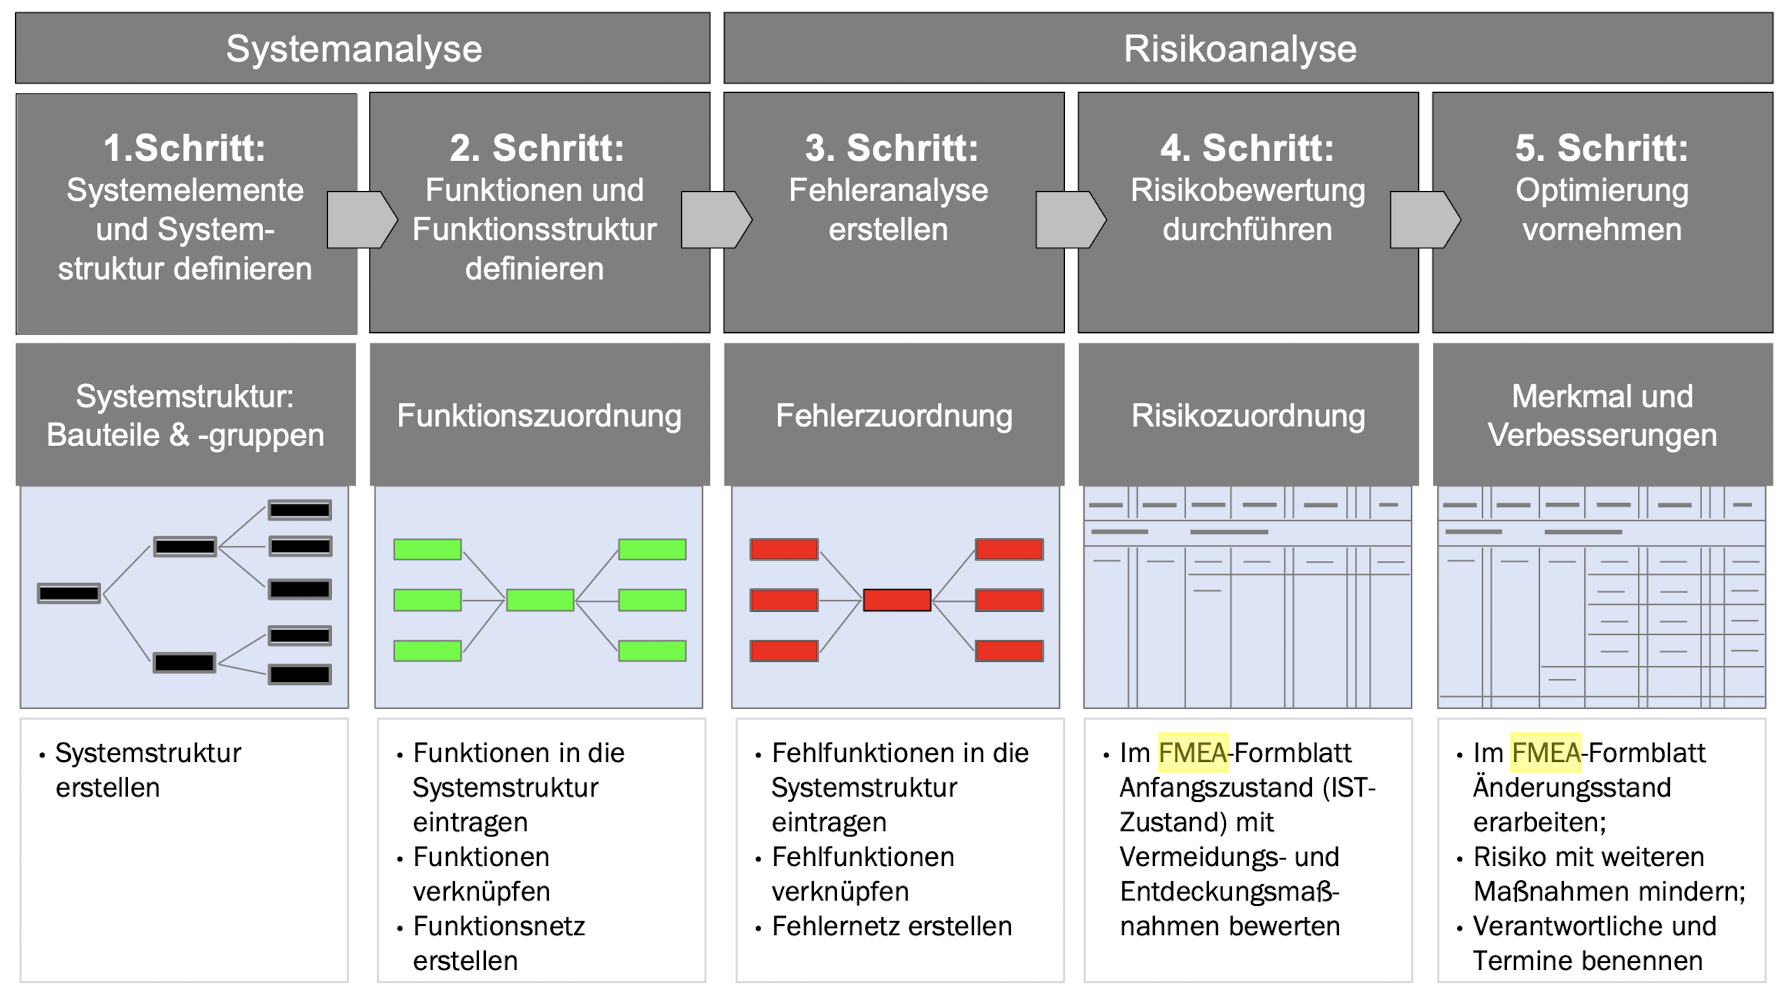
\includegraphics[width = 1.0\linewidth]{MAEIP_FMEA}
        \mathbox{
        RPZ = A \cdot B \cdot E \qquad A, B, E \in [1,10]
        }
        $RPZ$ = Risikoprioritätszahl, $A$ = Auftretenswahrscheinlichkeit, 
        \\$B$ = Bedeutung für Kunden, $E$ = Entdeckungswahrscheinlichkeit
        \\ \mathbox{RPZ < 100} $\to$ i.O. wenn Team Einzelwertung d. Risikozahlen akzeptiert
        \\\mathbox{100 < RPZ < 200} $\to$ Entscheidung im Ermessen d. Teams, Begründung notieren
        \\ \mathbox{A \in [1,10], \: B \in [1,10], \: E \in [10,1]}
        $\to$Wahrscheinlichkeiten tief-hoch
        \begin{empheq}[box=\fbox]{align*}
            RPZ > 200 \to \text{Definitive Massnahmexfer}
        \end{empheq}
        \begin{itemize}
            \item \textbf{Pro:} systematisch / universell anwendbar / einheitliche Dokumentation
            \item \textbf{Contra:} hoher Aufwand / Nutzen schwer quantifizierbar / unseriöses Durchführen ist einfach
        \end{itemize}
    \end{scriptsize}